\newpage
\addpart{Détection du tag}

    \section{Estimation de la matrice d'homographie}

    Bien qu'OpenCV dispose de méthodes pour estimer une matrice d'homographie entre deux jeux de points, nous avons décidé de réimplémenter une solution d'estimation d'homographie.

    La méthode d'estimation d'homographie se base sur la résolution d'un pivot de Gauss.

    On cherche pour chaque couple de points $p_i \leftrightarrow p_{i}' $ la matrice H telle que :

    $ p_i = Hp_i' $

    $ p_i $ correspondant aux points de départ.
    $ p'_i $ correspondant aux points d'arrivés.

    Soit pour tout point $i$ :

    \[
        \begin{bmatrix}
            x_i \\
            y_i \\
            1      
        \end{bmatrix}
        = 
        \begin{bmatrix}
            h1 &  h2 & h3 \\
            h4  & h5 & h6 \\
            h7 & h8 & h9      
        \end{bmatrix} 
        \times
        \begin{bmatrix}
            x'_i \\
            y'_i \\
            1      
        \end{bmatrix}
        \]
    
    L'objectif est donc de déterminer la matrice H telle que :

    \begin{center}
    $ H = \begin{pmatrix} h1 & h2 & h3 \\ h4 & h5 & h6 \\ h7 & h8 & h9 \end{pmatrix} $
    \end{center}

    Pour cela, on peut réécrire l'estimation de l'homographie pour un point de cette manière :

    $x_i = \frac{h1x'_i + h2y'_i + h3}{h7x'_i + h8y'_i + h9} $

    $y_i = \frac{h4x'_i + h5y'_i + h6}{h7x'_i + h8y'_i + h9} $

    Qui est égal à :

    $ x'_ih0 + y'_ih1 + h2 - x'_i x_ih7 - y'_ix_ih8 - x_ih9 = 0 $

    $ x'_ih3 + y'_ih4 + h5 - x'_iy_ih7 - y'_iy_ih8 - y_ih9 = 0 $

    Pour chaque point, nous avons donc deux équations qui permettent de résoudre $H$ sous la forme d'un système de 2 équations par point à 8 inconnues.

    Nous pouvons d'ailleurs par avance résoudre h9, car dans le cas d'une homographie, nous avons toujours $h9 = 1$.

    Il nous reste huit inconnues à résoudre : 4 points sont alors nécessaires pour générer 8 équations dans le système, dont on considère $h9$ comme déjà résolu : 

    \[
      \begin{pmatrix} 
        x_1 & y_1 & 1 & 0 & 0 & 0 & -x_1 x'_1 & -y_1 x'_1 \\ 
        0 & 0 & 0 & x_1 & y_1 & 1 & -x_1 y'_1 & -y_1 y'_1 \\

        x_2 & y_2 & 1 & 0 & 0 & 0 & -x_2 x'_2 & -y_2 x'_2 \\ 
        0 & 0 & 0 & x_2 & y_2 & 1 & -x_2 y'_2 & -y_2 y'_2 \\

        x_3 & y_3 & 1 & 0 & 0 & 0 & -x_3 x'_3 & -y_3 x'_3 \\ 
        0 & 0 & 0 & x_3 & y_3 & 1 & -x_3 y'_3 & -y_3 y'_3 \\

        x_4 & y_4 & 1 & 0 & 0 & 0 & -x_4 x'_4 & -y_4 x'_4 \\ 
        0 & 0 & 0 & x_4 & y_4 & 1 & -x_4 y'_4 & -y_4 y'_4
    \end{pmatrix} 
    \times
    \begin{pmatrix} h1 \\ h2 \\ h3 \\ h4 \\ h5 \\h6 \\ h7 \\ h8 \end{pmatrix}
    =
    \begin{pmatrix} x'_1 \\ y'_1 \\ x'_2 \\ y'_2 \\ x'_3 \\ y'_3 \\ x'_4 \\ y'_4 \end{pmatrix} 
    \]

    Un pivot de Gauss est réalisé sur ce système d'équations. Une fois ce pivot résolu, nous obtenons une matrice en "row echelon form", c'est à dire :

    \begin{itemize}
        \item Toutes les lignes qui ne sont pas entièrement constituées de 0 commencent par un 1
        \item Pour deux lignes non constituées que de 0, la valeur 1 de la ligne placée en haut de la matrice sera plus à gauche que le 1 de la ligne placée plus bas
        \item Toutes les lignes avec seulement des 0 sont placées en bas
    \end{itemize}

    Nous effectuons en conséquence une "back substitution" pour faire apparaître la solution sur la dernière colonne.

    La dernière colonne du système est donc la résolution de la matrice H, qui nous donne notre matrice d'homographie.

    \section{Amélioration de la détection du tag}

    Après les premiers tests, nous avons remarqué que la détection du tag était efficiente lorsque le tag était bien visible quel que soit sa rotation ou sa taille, mais perdait en efficacité lors de mouvements plus brusques de la caméra, notamment à cause du flou de mouvement.

    Nous avons implémenté deux méthodes pour rendre plus robuste cette détection afin de détecter le tag même lors des mouvements de la caméra.

        \subsection{Défloutage gaussien}

        Une première méthode pour optimiser la détection du tag est de retirer le bruit causé par le flou de mouvement de la caméra lorsque le tag n'est pas détecté.

        Pour cela, on va considérer que le flou est causé par un flou gaussien. L'objectif est de soustraire l'image floutée par sa propre image non floutée.

        Nous appliquons un flou gaussien sur l'image bruitée. Ensuite, nous calculons la somme pondérée de l'image d'entrée et l'image floutée, avec un poids de $1.5$ pour l'image d'entrée et un poids de $-0.5$ pour l'image floutée. Nous prenons en réalité l'image bruitée par le flou de mouvement, auquel nous soustrayons l'image floutée par le filtre gaussien. Ceci permet d'éliminer une partie du flou sur l'image original et d'affiner les contours.

        \subsection{Marge d'acceptation de détection du tag}

        Comme nous l'avons vu précédemment, chaque tag potentiel détecté sur l'image est comparé au modèle de tag pour vérifier si les 64 cases du candidat correspondent bien au tag que nous cherchons.

        Lors du mouvement de la caméra, il peut arriver que le flou de mouvement empiète sur certaines cases et modifie légèrement le résultat, ce qui en conséquence écarte le tag de la recherche.

        Nous pouvons en conséquence tolérer un seuil d'acceptation du tag, où si jamais entre 5 et 10 \% des cases du potentiel tag ne corrèlent pas au modèle, le candidat est quand même accepté comme étant le tag, car si observons une correspondance par exemple sur 56 cases du tag sur les 64, nous pouvons être quasiment sûr qu'il s'agit bien du tag que nous recherchons.

        \subsection{Résultats}

        Les deux méthodes indépendamment améliorent, mais pas de façon considérable les résultats, mais en les combinant nous parvenons à avoir une détection plus robuste.

        \begin{figure}[!h]
            \begin{center}
                \begin{tabular}{ | c | c | c | c | c | }
                \hline
                Vidéo & Sans optimisation & Approximation & Défloutage Gaussien & Combinaison \\ \hline
                Vidéo 1 & 88.2\% & 91.4\% & 90.9\% & 94.1\% \\ \hline
                Vidéo 2 & 12.21\% & Non testé & Non testé & 37.40\% \\
                \hline
                \end{tabular}
        \end{center}
        \caption{Taux de détection du tag par vidéo}
        \end{figure}

        Vidéo 1 : Vidéo de plutôt bonne qualité, le tag sort de l'écran une seconde

        Vidéo 2 : Vidéo de mauvaise qualité, plus de mouvement de la caméra, le tag est plus petit et légèrement froissé.

        Bien que la détection avec ces méthodes reste généralement de bonne qualité, il y a malgré tout plus de risque d'avoir une détection d'être dégradée, comme il peut être observé sur l'image ci-dessous.

        \begin{figure}[!h]
            \centering
            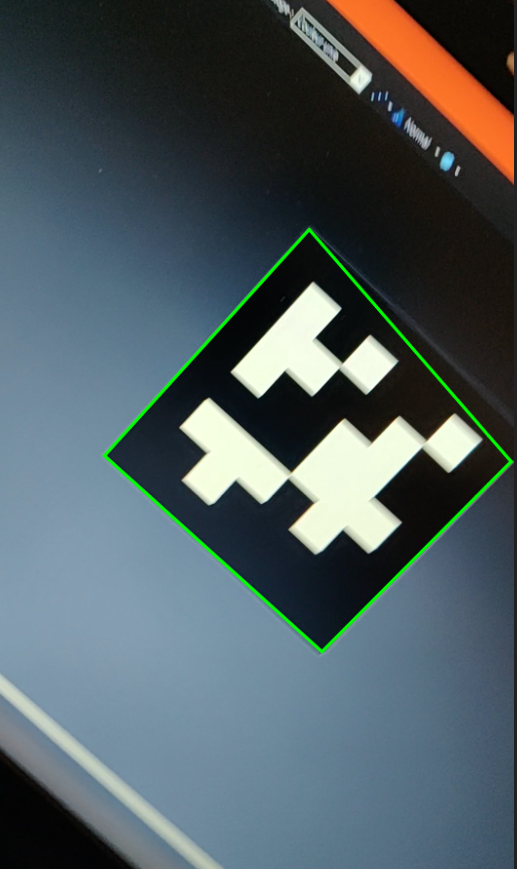
\includegraphics[scale=0.25]{img/cropped_tag.png}
            \caption{Le tag est détecté, mais un angle n'est pas bien géré}
        \end{figure}

        Pour éviter de dégrader la détection des contours lors des frames suivantes du flux vidéo, nous ne réalisons pas de tracking sur le tag que nous avons détecté à l'aide des méthodes d'optimisations, car il sera éventuellement possible de trouver un tag parfait lors de la frame suivante, qui serait de meilleur qualité qu'un tag de moins bonne qualité tracké par rapport à celui de la frame précédante.

        De plus, ces méthodes d'optimisations ne permettent pas de détecter le tag lorsqu'il sort de l'écran.